\documentclass[12pt]{amsart}
\usepackage{geometry} % see geometry.pdf on how to lay out the page. There's lots.
\usepackage{graphicx}	% Including figure files
\usepackage{amsmath}	% Advanced maths commands
\usepackage{amssymb}	% Extra maths symbols
\usepackage{hyperref}
\geometry{a4paper} % or letter or a5paper or ... etc

\title{CSE 546 HW1}
\author{David P. Fleming}
\date{October 14$^{th}$, 2016}

%%% BEGIN DOCUMENT
\begin{document}

\maketitle
\tableofcontents

\section*{Introduction}

Please note that a copy of all the code I wrote to answer the questions in this assignment are included in my submission but also located online at \url{https://github.com/dflemin3/CSE_546/tree/master/HW1}.  Some scripts require data, be it MNIST or Yelp, to run to completion and were not included on my github or in my submission due to file size constraints.  If requested, I will happily send a compressed directory containing my homework and detailed instructions on how to reproduce my work.  My primary email is dflemin3 (at) uw (dot) edu.  Also for reproducibility, I set the random number generator seed near the top of each script such that rerunning my script will yield the same answers as presented here.

%%% QUESTION 1 %%%

\section*{Question 1: Probability}

\subsection*{1.1}
The expectation value for $max(X_1, X_2)$ is given by
\begin{align}
E[X] = \int max(X_1,X_2) f(x) dx_1 dx_2
\end{align}
where $f(x) = 1$ is the PDF for the uniform random variates.  We consider two regions, one below the line defined by $X = X_1 = X_2$ and one above said line for our integrations.  This gives us the following integral:

\begin{equation} \label{eqn:1.1}
\begin{split}
E[X] & = \int_0^1 \int_{x_2}^1 x_1 dx_1 dx_2 + \int_0^1 \int_{x_1}^1 x_2 dx_2 dx_1 \\
& = \int_0^1 (\frac{1}{2} - \frac{1}{2}x_2^2) dx_2 + \int_0^1 (\frac{1}{2} - \frac{1}{2}x_1^2) dx_1 \\
& = (\frac{1}{2}x_2 - \frac{1}{6}x_2^2) \vert_0^1 + (\frac{1}{2}x_1 - \frac{1}{6}x_1^2) \vert_0^1 \\
& = \frac{2}{3}
\end{split}
\end{equation}

\subsection*{1.2}
Since
\begin{align}
Var[X] = E[X^2] - E[X]^2
\end{align}
and we now know $E[X] = 2/3$, we solve the integral presented above but with the integrand squared as follows
\begin{equation} \label{eqn:1.2}
\begin{split}
E[X^2] & = \int_0^1 \int_{x_2}^1 x_1^2 dx_1 dx_2 + \int_0^1 \int_{x_1}^1 x_2^2 dx_2 dx_1 \\
& = \int_0^1 (\frac{1}{3} - \frac{1}{3}x_2^3) dx_2 + \int_0^1 (\frac{1}{3} - \frac{1}{3}x_1^3) dx_1 \\
& = (\frac{1}{3}x_2 - \frac{1}{12}x_2^4)\vert_0^1 + (\frac{1}{3}x_1 - \frac{1}{12}x_1^4)\vert_0^1 \\
& = \frac{1}{2}
\end{split}
\end{equation}

which when combined with the definition for $Var[X]$ gives
\begin{equation}
Var[X] = \frac{1}{2} - \left( \frac{2}{3} \right)^2 = \frac{1}{18}
\end{equation}

\subsection*{1.3}

Since 
\begin{align}
Cov[X,X_1] = E[X X_1] - E[X]E[X_1]
\end{align}
and we know $E[X]$ from $1.1$ and $E[X_1] = 1/2$ is the trivial result for the uniform distribution from $[0,1]$, we need only calculate the first term as follows:
\begin{equation} \label{eqn:1.3}
\begin{split}
E[XX_1] & = \int_0^1 \int_{x_2}^1 x_1^2 dx_1 dx_2 + \int_0^1 \int_{x_1}^1 x_2 x_1 dx_2 dx_1 \\
& = \int_0^1 (\frac{1}{3} - \frac{1}{3}x_2^3) dx_2 + \int_0^1 x_1(\frac{1}{2} - \frac{1}{2}x_1^2) dx_1 \\
& = (\frac{1}{3}x_2 - \frac{1}{12}x_2^4) \vert_0^1 + (\frac{1}{4}x_1^2 - \frac{1}{8}x_1^4) \vert_0^1 \\
& = \frac{3}{8} 
\end{split}
\end{equation}
giving us
\begin{equation}
Cov[X,X_1] = E[X X_1] - E[X]E[X_1] = \frac{3}{8} - \frac{2}{3}\frac{1}{2} = \frac{1}{24}
\end{equation}

Note: For this question, I collaborated with Matt Wilde.

%%% QUESTION 2 %%%
\section*{Question 2: MLE}

\subsection*{2.1}

For the log-likelihood of G given $\lambda$ and i.i.d. samples, we have
\begin{equation} \label{eqn:2.1}
\begin{split}
LL & = \log \left( P(G | \theta)  \right) \\
& = \Pi_i^n P(G_i | \theta) \\
& = \log \left( \frac{\lambda^{\Sigma_i^n k_i} e^{-\lambda n}}{\Pi_i^n k_i !} \right) \\
& = \Sigma_i^n k_i \log \lambda - \lambda n - \log \Pi_i^n k_i !
\end{split}
\end{equation}

\subsection*{2.2}

To compute the MLE for $\lambda$ in general,
\begin{equation} 
\begin{split}
\frac{\partial}{\partial \lambda} \left[ LL \right] = 0
\end{split}
\end{equation}
which yields

\begin{equation} \label{eqn:2.2}
\begin{split}
0 & = \frac{\partial}{\partial \lambda} \left( \Sigma_i^n k_i \log \lambda - \lambda n - \log \Pi_i^n k_i ! \right) \\ 
& = \frac{\Sigma_i^n k_i}{\lambda} - n \\
\hat{\lambda}_{MLE} & = \frac{\Sigma_i^n k_i}{n} \\
\end{split}
\end{equation}

\subsection*{2.3}
For the observed set G, I use Eqn.~\ref{eqn:2.2} to compute $\lambda_{MLE}$ as
\begin{equation}
\hat{\lambda}_{MLE} = \frac{4+1+3+5+5+1+3+8}{8} = 3.75
\end{equation}

Note: For this question, I collaborated with Matt Wilde.

%%% QUESTION 3 %%%

\section*{Question 3: Linear Regression and LOOCV}

\subsection*{3.1}

To compute the LOOCV score natively, one must compute $\hat{y}$ $N-1$ times where $\hat{y}$ is the prediction vector computed via Ordinary Least-Squares (OLS).  Therefore, the time complexity of computing LOOCV will be $\mathcal{O}(N * \mathcal{O}(OLS))$.  To compute $\mathcal{O}(OLS)$, I will assume the naive algorithm for matrix inversion which has complexity $\mathcal{O}(d^3)$ for a $d \times d$ matrix and assume the naive algorithm for matrix multiplication which has complexity $\mathcal{O}(nmp)$ for the matrix product of $n \times m$ and $m \times p$ matrices.

For OLS, $\hat{Y_{OLS}} = X(X^T X)^{-1}X^T Y$ where $X$ is $N \times d$ and $Y$ is $N \times 1$.  The complexities of taking multiple matrix products sum since they happen sequentially.  If we take the pairwise matrix products to compute $\hat{Y_{OLS}}$, we get $\mathcal{O}(Nd^2)$ + $\mathcal{O}(Nd^2)$ + $\mathcal{O}(dN^2)$ + $\mathcal{O}(N^2)$.  Combining those terms with the $\mathcal{O}(d^3)$ complexity addition from matrix inversion, I get a total complexity of $\mathcal{O}(d^3 + (1+2d)N^2 + Nd^2)$ which asymptotes to $\mathcal{O}(d^3 + dN^2 + Nd^2)$.  If $N > d$, this term can be reduced further however I make no assumptions about whether $d$ or $N$ is larger.  To compute LOOCV, we must compute $\hat{Y}$ $N - 1$ times giving a total complexity of $\mathcal{O}(Nd^3 + dN^3 + N^2d^2)$.

\subsection*{3.2}

Since in matrix notation we have $\hat{Y} = HY$, I can write 
\begin{equation}
\hat{y_i} = \sum_{j=1}^N H_{ij}y_j
\end{equation}
where $\hat{y}$ has length $N$.

\subsection*{3.3}

To show that $\hat{Y}^{(-i)}$ is the estimator which minimizes SSE for the given $Z_j$, first I substitute $Z_j$ for $y_i$ in the given expression for SSE to get the following
\begin{equation}
SSE = \sum_{j=1}^N (Z_j - \hat{y_j})^2.
\end{equation} 

Now, I expand the above expression for SSE using the definition of $Z_j$

\begin{equation}
\begin{split}
SSE & = \sum_{j \neq i}^N (y_j - \hat{y_j})^2  + (\hat{y}_i^{(-i)} - \hat{y_i})^2
\end{split}
\end{equation}
which reduces to the original SSE with an additional $i = j$ term.  Therefore $\hat{Y}^{(-i)}$ must be the estimator which minimizes the SSE for $Z$.

\subsection*{3.4}

Analogous to the answer to Question 3.2, I can write $\hat{Y}^{(-i)} = HZ$ or in summation notation,
\begin{equation}
\hat{y}_i^{(-i)} = \sum_{j = 1}^N H_{ij}Z_j
\end{equation}

\subsection*{3.5}

To show that $\hat{y}_i - \hat{y}_i^{(-i)} = H_{ii}y_i - H_{ii}\hat{y}_i^{(-i)} $, I will take the left-hand side (LHS) of the equation and expand it with my definitions for $\hat{y}_i $ and $\hat{y}_i^{(-i)}$ from my answers to 3.2 and 3.4 as follows

\begin{equation}
\begin{split}
\hat{y}_i - \hat{y}_i^{(-i)}  & = \\
\sum_{j = 1}^N H_{ij}y_j - \sum_{j = 1}^N H_{ij}Z_j & = \\
\sum_{j \neq i}^N H_{ij}y_j + H_{ii}y_i - \sum_{j \neq i}^N H_{ij}y_j - H_{ii}\hat{y}_i^{(-i)} & = \\
H_{ii}y_i - H_{ii}\hat{y}_i^{(-i)} & = RHS
\end{split}
\end{equation}
as the $j \neq i$ term in $Z_j$ allows us to cancel the summation terms, giving us the RHS as posited.

\subsection*{3.6}

To derive the expected result, first I will rearrange $\hat{y}_i - \hat{y}_i^{(-i)} = H_{ii}y_i - H_{ii}\hat{y}_i^{(-i)}$ as follows
\begin{equation}
\begin{split}
\hat{y}_i - \hat{y}_i^{(-i)} & = H_{ii}y_i - H_{ii}\hat{y}_i^{(-i)}  \\
\hat{y}_i - H_{ii}y_i & =  \hat{y}_i^{(-i)} - H_{ii}\hat{y}_i^{(-i)} \\
\hat{y}_i - H_{ii}y_i & =  (1 - H_{ii})\hat{y}_i^{(-i)} \\
\hat{y}_i^{(-i)} & = (\hat{y}_i - H_{ii}y_i) \frac{1}{1 - H_{ii}}.
\end{split}
\end{equation} 
I now insert this expression for $\hat{y}_i^{(-i)}$ into the expression for LOOCV and reduce to derive the following
\begin{equation}
\begin{split}
LOOVC & = \sum_{i = 1}^N (y_i - \hat{y}_i^{(-i)})^2 \\
& = \sum_{i = 1}^N \left( y_i -  (\hat{y}_i - H_{ii}y_i) \frac{1}{1 - H_{ii}} \right)^2 \\
& = \sum_{i = 1}^N \left( y_i\frac{1 - H_{ii}}{1 - H_{ii}} -  \frac{\hat{y}_i}{1 - H_{ii}}  + \frac{H_{ii}y_i}{1 - H_{ii}}  \right)^2 \\
& = \sum_{i = 1}^N \left( \frac{y_i - \hat{y_i}}{1 - H_{ii}} \right)^2.
\end{split}
\end{equation}

With the updated formula, we can estimate the naive algorithmic complexity of computing the LOOCV by noting that we need only compute $\hat{Y_{OLS}}$ once this time.  We get the $H$ term as a part of the $\hat{Y}$ computation.  Therefore, the algorithmic complexity of the LOOCV using the new formula is equal to that of the OLS I derived above and is given by $\mathcal{O}(d^3 + dN^2 + Nd^2)$.

Note for this question, I collaborated with Matt Wilde and Serena Liu.

%%% QUESTION 4 %%%

\section*{Question 4: Regularization Constant}

Note: Both both subquestions 1 and 2, I assume that the too small or too large $\lambda$s bias the model to a too complex or too simple model relative to the optimum model complexity, respectively.

\subsection*{4.1: Too Small a $\lambda$}
\subsubsection*{4.1.a}
For both LASSO and Ridge Regression (RR), the error on the training set would decrease as the penalty term for both regression techniques would be effectively negligible.  With small $\lambda$, the regularization penalty is also small causing both regression techniques to tend towards least squares regression (LSR) and allow for more complex models which overfit the training data and hence leading to smaller training set error.  For example, too small of a $\lambda$ could push both LASSO and RR to favor a high-order polynomial model when the underlying data is linear.

\subsubsection*{4.1.b}
For both LASSO and RR, too small a $\lambda$ leads to overfitting on the training set.  With a model overfit on the training set, it will do a poor job of generalizing to new data and hence will poorly fit the testing set leading to larger testing error.

\subsubsection*{4.1.c}
For both LASSO and RR, too small a $\lambda$ yields too small of a complexity penalty causing both algorithms to tend towards the LSR solution.  In this case, $\hat{\omega}$ could get large via overfitting.  RR, however, will likely predict larger $\hat{\omega}$ than LASSO as RR's $l_2$ norm penalty primarily seeks to control the magnitude of the weight vector, hence biasing towards larger values in this case as the penalty decreases, while LASSO seeks a sparse solution.


\subsubsection*{4.1.d}
With LASSO, too small of a $\lambda$ would yield more non-zero parameters since a smaller regularization penalty will prevent many of the elements of $\hat{\omega}$ from being set to 0 under LASSO's sharp $l_1$ norm penalty which tries to make $\hat{\omega}$ sparse.  For RR, too small of a $\lambda$ would have little effect on the number of non-zero parameters as RR's regularization penalty deals with constraining the magnitude of $\hat{\omega}$ as opposed to forcing it to be sparse.

\subsection*{4.2: Too Large a $\lambda$}
\subsubsection*{4.2.a}
For both regression techniques, too large of a $\lambda$ will yield larger training set error as the regularization penalty will select for simpler models that could poorly fit the data.  For example, too large of a $\lambda$ could push both LASSO and RR to favor a linear model when the underlying data is quadratic.

\subsubsection*{4.2.b}
For both LASSO and RR, too large of a $\lambda$ will yield larger testing set error since the models again will be biased towards lower-than-optimal model complexity and hence will likely yield a poor fit to future data similar to why the error on the training set is also larger in this case.

\subsubsection*{4.2.c}
For both LASSO and RR, too large of a $\lambda$ will yield smaller $\hat{\omega}$ as the larger regularization penalty restricts the weight vector.  RR, however, will likely predict smaller $\hat{\omega}$ than LASSO as RR's $l_2$ norm penalty primarily seeks to control the magnitude of the weight vector, hence biasing towards smaller values in this case, while LASSO seeks a sparse solution.

\subsubsection*{4.2.d}
For LASSO, a larger $\lambda$ will yield a sparser solution via its $l_1$ norm regularization penalty and hence will have fewer nonzero elements in $\hat{\omega}$ than RR.  In the large $\lambda$ limit, RR will also yield fewer nonzero elements in $\hat{\omega}$ only because its large regularization penalty makes coefficients in its weight vector small and hence potentially pushing some towards 0.

Note: For this question, I collaborated with Matt Wilde.

%%% QUESTION 5 %%%

\section*{Question 5: Regression and Agnostic Learning}

\subsection*{5.1: Bayes Optimal Prediction}

\subsubsection*{5.1.1}

For the following derivation, I will make use of the following conditional probability identities

\begin{equation} \label{eqn:exp_rule_1}
E_{X,Y}[arg] = E_{X}[E_{Y|X}[arg]]
\end{equation}
for some arbitrary argument $arg$ and 
\begin{equation} \label{eqn:exp_rule_2}
E_{Y|X}[Y] = E[Y|X]
\end{equation}
which is the Law of Iterated Expectations.

Now, I first write $L(f)$ and add a form of 0 and expand the terms as follows
\begin{equation} \label{eqn:bayes_reg}
\begin{split}
L(f) & = E_{X,Y}[(Y - f(X))^2] \\
& = E_{X,Y}[((Y - E[Y|X]) + (E[Y|X] - f(X)))^2] \\
& = E_{X,Y}[(Y - E[Y|X])^2 + (E[Y|X] - f(X))^2 - 2(Y - E[Y|X])(E[Y|X] - f(X))] .
\end{split}
\end{equation}
To simplify Eqn.~\ref{eqn:bayes_reg}, I will split it up into 3 terms.  Note that the first term, $E_{X,Y}[(Y - E[Y|X])^2]$ is the second term in the answer, so I will leave that be.  

The second term can be simplified as follows
\begin{equation}
\begin{split}
& E_{X,Y}[(E[Y|X] - f(X))^2] \\
& = E_X[E_{Y|X}[(E[Y|X] - f(X))^2]] \\
& = E_X[(E[Y|X] - f(X))^2]
\end{split}
\end{equation}
via Eqn.~\ref{eqn:exp_rule_1} and since both $E[Y|X]$ and $f(X)$ are constant with respect to (wrt) integration over $Y$.  Now, we have
\begin{equation}
E_{X,Y}[(Y - E[Y|X])^2] + E_X[(E[Y|X] - f(X))^2] - E_{X,Y}[2(Y - E[Y|X])(E[Y|X] - f(X))]
\end{equation}
and need only shown that the third term in the above relation goes to 0 to complete the proof which I do below (Note: I use f instead of f(X) for brevity)
\begin{equation}
\begin{split}
& E_{X,Y}[(Y - E[Y|X])(E[Y|X] - f(X))] \\
& = E_{X,Y}[YE[Y|X] - Yf - E[Y|X]^2 + fE[Y|X]] \\
& = E_{X,Y}[YE[Y|X] - E[Y|X]^2 + fE[Y|X] - Yf] \\
& = E_X[E_{Y|X}[YE[Y|X]] - E_{Y|X}[E[Y|X]^2] + E_{Y|X}[fE[Y|X]] - E_{Y|X}[Yf]] \\
& = E_X[E_{Y|X}[Y]E[Y|X] - E[Y|X]^2 + fE[Y|X] - E_{Y|X}[Y]f] 
\end{split}
\end{equation}
where I used the fact that both $f$ and $E[Y|X]$ do not depend on $Y$ and hence $E_{Y|X}[E[Y|X]] = E[Y|X]$ and $E_{Y|X}[f] = f$.  Now using Eqn.~\ref{eqn:exp_rule_2}, 
\begin{equation}
\begin{split}
& E_X[E_{Y|X}[Y]E[Y|X] - E[Y|X]^2 + fE[Y|X] - E_{Y|X}[Y]f] \\
& = E_X[E[Y|X]^2 - E[Y|X]^2 + fE[Y|X] - E[Y|X]f] \\
& = 0
\end{split}
\end{equation}
and completing the proof.

\subsubsection*{5.1.2}
Given the expression derived above for the square loss for a function $f$, the Bayes optimal regressor $f_{Bayes} = E[Y|X]$.  This expression for $f_{Bayes}$ is the optimal regressor because the best function one can learn from the data given a class of learnable functions is the expected value of the label given the data, $E[Y|X]$ .  With the expression for $f_{Bayes}$, I get 
\begin{equation}
\begin{split}
L(f_{Bayes}) & = E_X[E[Y|X] - f_{Bayes}^2] + E_{X,Y}[(Y - E[Y|X])^2] \\
& = E_X[(E[Y|X] - E[Y|X])^2] + E_{X,Y}[(Y - E[Y|X])^2] \\
& = E_{X,Y}[(Y - E[Y|X])^2].
\end{split}
\end{equation}
This expression for $L(f_{Bayes})$ represents the inherent uncertainty in the data which sets the error limit a model cannot improve upon.

\subsection*{5.2: Bias-Variance-Noise Error Decomposition}

\subsubsection*{5.2.1}

For this proof I will use, in addition to the Eqns.~\ref{eqn:exp_rule_1,eqn:exp_rule_2}, the following given expression
\begin{equation} \label{eqn:fhat_fbar}
\bar{f}(X) = E_T[\hat{f}(X)]
\end{equation}
where $\bar{f}(X)$ is the expected function wrt the randomness in our training set T.  $E_T[L(\hat{f})]$ us then the expected square loss of our estimation procedure wrt to the training set T.

To derive the final result I first foil the expression and expand
\begin{equation} \label{eqn:et_lf_0}
\begin{split}
E_T[L(\hat{f})] & = E_TE_{X,Y}[(Y - \hat{f})^2] \\
& = E_TE_{X,Y}[Y^2 - 2y\hat{f} + \hat{f}^2] \\
& = E_TE_{X,Y}[Y^2] - 2E_TE_{X,Y}[Y\hat{f}] + E_TE_{X,Y}[\hat{f}^2]
\end{split}
\end{equation}
where $\hat{f} = \hat{f}(X)$ for brevity.  To simplify, I will tackle this expression piece-wise and regroup later.  First, I manipulate the 3rd term as follows
\begin{equation} \label{eqn:fhat_var}
\begin{split}
& E_TE_{X,Y}[\hat{f}^2] \\
& = E_TE_{X,Y}[(\hat{f} - E_{X,Y}E_T[\hat{f}])^2] + E_TE_{X,Y}[\hat{f}]^2 \\
& = E_TE_{X,Y}[(\hat{f} - \bar{f})^2] + E_TE_{X,Y}[\hat{f}]^2 \\
& = E_TE_{X,Y}[(\hat{f} - \bar{f})^2] + E_{X,Y}E_T[\hat{f}]^2 \\
& = E_TE_{X,Y}[(\hat{f} - \bar{f})^2] + E_{X,Y}[\bar{f}]^2 \\
& = E_TE_{X,Y}[(\hat{f} - \bar{f})^2] + \bar{f}^2
\end{split}
\end{equation}
since $Var[X] = E[(X - E[X])^2] = E[X^2] - E[X]^2$ and given Eqn.~\ref{eqn:fhat_fbar}.  Also, I used the fact that $\bar{f}$ is constant wrt any integration over the underlying distribution and hence any expectation of $\bar{f}$ over $X,Y$ is just $\bar{f}$.  In addition, I note that $E_T$ is taking the expectation with respect the the randomness in the training set via the variance from sampling X and Y. This variance between draws is independent of the underlying distribution allowing me to treat T and X,Y as independent random variables allowing me to switch the order of expectations from $E_T E_{X,Y}$ to $E_{X,Y}E_T$.

Now in the above Eqn.~\ref{eqn:fhat_var}, we see that the first term, $E_TE_{X,Y}[(\hat{f} - \bar{f})^2]$, is the first term in the answer, so we will suggestively denote it as $Var$ for now for brevity.  Recombining Eqn.~\ref{eqn:fhat_var} and Eqn.~\ref{eqn:et_lf_0} and simplifying yields
\begin{equation} \label{eqn:et_lf_1}
\begin{split}
& E_TE_{X,Y}[Y^2] - 2E_TE_{X,Y}[Y\hat{f}]  + \bar{f}^2 + Var \\
& = E_TE_{X,Y}[Y^2] - 2E_{X,Y}[YE_T[\hat{f}]] + E_{X,Y}[\bar{f}^2] + Var \\
& = E_{X,Y}E_T[Y^2] - 2E_{X,Y}[YE_T[\hat{f}]] + E_{X,Y}[\bar{f}^2] + Var \\
& = E_{X,Y}[Y^2 - 2Y\bar{f} +  \bar{f}^2] + Var \\
& = E_{X,Y}[(Y - \bar{f})^2] + Var \\
\end{split}
\end{equation}
where I also used $E_T[Y] = Y$.  Now, I add a form of 0 and expand again
\begin{equation} \label{eqn:et_lf_02}
\begin{split}
& E_{X,Y}[((Y - E[Y|X]) + (E[Y|X] - \bar{f}))^2] + Var \\
& = E_{X,Y}[(Y-E[Y|X])^2] + E_{X,Y}[(E[Y|X] - \bar{f})^2] - 2E_{X,Y}[(Y-E[Y|X])((E[Y|X] - \bar{f})] + Var \\
& = E_{X,Y}[(Y-E[Y|X])^2] + E_{X,Y}[(E[Y|X] - \bar{f})^2]  + E_TE_{X,Y}[(\hat{f} - \bar{f})^2]  \\
& - 2E_{X,Y}[(Y-E[Y|X])((E[Y|X] - \bar{f})].
\end{split}
\end{equation}
Note that the first term in this expression, $E_{X,Y}[(Y-E[Y|X])^2]$, appears in the answer so I will leave it as-in.  The second and third terms, $E_{X,Y}[(E[Y|X] - \bar{f})^2]  + E_TE_{X,Y}[(\hat{f} - \bar{f})^2]$, are close to terms in the answer so I will simplify them next.

\begin{equation} 
\begin{split}
& E_{X,Y}[(E[Y|X] - \bar{f})^2] \\
& = E_X[E_{Y|X}[(E[Y|X] - \bar{f})^2]] \\
& = E_X[(E[Y|X] - \bar{f})^2]
\end{split}
\end{equation}
via Eqn.~\ref{eqn:exp_rule_1}.  This gives us another term from the final answer, so I will leave it as-in.  Now for the other term
\begin{equation}
\begin{split}
& E_TE_{X,Y}[(\hat{f} - \bar{f})^2] \\
& = E_TE_X[E_{Y|X}[(\hat{f} - \bar{f})^2]] \\
& = E_TE_X[(\hat{f} - \bar{f})^2]
\end{split}
\end{equation}
since both $\hat{f}$ and $\bar{f}$ are constant wrt integration over the underlying distribution in $Y$.  Collecting terms again, we have
\begin{equation} \label{eqn:5.2almost_ans}
\begin{split}
&E_TE_X[(\hat{f} - \bar{f})^2] + E_X[(E[Y|X] - \bar{f})^2] + E_{X,Y}[(Y-E[Y|X])^2] \\
& - 2E_{X,Y}[(Y-E[Y|X])((E[Y|X] - \bar{f})]
\end{split}
\end{equation}
which is the answer minus an additional term.  Below, I show that the additional term goes to 0, completing the proof.  Expanding the final term and noting that $E_{X,Y}[Y] = E[Y|X]$, 
\begin{equation}
\begin{split}
& E_{X,Y}[(Y-E[Y|X])((E[Y|X] - \bar{f})] \\
& = E_{X,Y}[YE[Y|X] - Y\bar{f} - E[Y|X]^2 + \bar{f}E[Y|X]] \\
& = E[Y|X]E_{X,Y}[Y] - \bar{f}E_{X,Y}[Y] - E[Y|X]^2 + \bar{f}E[Y|X] \\
& = E[Y|X]^2 - \bar{f}E[Y|X] - E[Y|X]^2 + \bar{f}E[Y|X] \\
& = 0
\end{split}
\end{equation}
which completes the proof.

\subsubsection*{5.2.2}
The bias term which represents the difference between what you expect to learn, $\bar{f}$, and the the true solution, $E[Y|X]$, is given by the following term: $E_X[(E[Y|X] - \bar{f})^2]$.  Variance, or the difference between what you expect to learn, $\bar{f}$, and what you actually learn from a dataset, $\hat{f}$, is given by $E_TE_X[(\hat{f} - \bar{f})^2]$.  Finally the error term given by $E_{X,Y}[(Y-E[Y|X])^2]$ is the difference between the dependent variable and the true solution.

\subsubsection*{5.2.3}
For the empirical risk minimizer (ERM), $f^{*} \neq \bar{f}$.

\subsubsection*{5.2.4}
In the large sample size limit, I expect $\hat{f}$ to converge to $\bar{f}$ since $E_T[\hat{f}] = \bar{f}$ since sampling over large number of points will effectively marginalize over the randomness of the training sets.  Also, I expect $\bar{f}$ to converge towards $f^{*}$ since in the large sample limit, the expected value will tend towards the truth.

Note: For this question, I collaborated with Matt Wilde and Serena Liu.

%%% QUESTION 6 %%%

\section*{Question 6: Classification Using Least Squares}

Note: The following scripts (attached) include all code used to solve this question: {\tt hw1$\_$6.py, mnist$\_$utils.py, regression$\_$utils.py, ridge$\_$utils.py, validation.py}.

Here, the I build a linear classifier by minimizing the following Ridge Regression Loss:
\begin{equation} \label{eqn:RR_loss}
\text{min}_{\omega} = \frac{1}{N} \sum_{i = 1}^N (y_i - \omega \cdot x_i)^2 + \lambda || \omega ||^2.
\end{equation}
In general, the RR regression weight vector can be solved for analytically via the following
\begin{equation} \label{eqn:RR_w}
\hat{\omega_{ridge}} = (\lambda I_D + X^T X)^{-1} X^T y
\end{equation}
however the matrix inversion required is not only computationally expensive but also can be numerically unstable.  Instead, I minimize Equation~\ref{eqn:RR_loss} by following the formulae in the textbook (see Murphy Section 7.5.2) which involves centering the data and augmenting X with the Cholesky decomposition of the precision matrix and y with a vector of 0s.  This yields the MAP estimate
\begin{equation} \label{eqn:RR_w_murphy}
\hat{\omega_{ridge}} = (\tilde{X}^T \tilde{X})^{-1} \tilde{X}^T \tilde{y}.
\end{equation}
This formula allows me to quickly solve the ridge regression problem for a given $\lambda$.

\subsection*{6.1: Binary Classification with Regression}

The hyperparameters of my model, the regularization parameter $\lambda$ and the threshold parameter $c$, were simultaneously fit for along a regularization grid.  Since my training set was sufficiently large with $N = 60,000$ samples, I randomly partitioned it into a validation set with $N_{val} = 6,000$ and a training set with $N_{train} = 54,000$.  I iterated over a two-dimensional grid of thresholds $c \in [-0.2,1]$ in 20 linear bins and $\lambda \in [10^{-5},10^{10}]$ in 20 logarithmic bins.  For each $(c,\lambda)$ pair, I fit the ridge regression on the training set then tested it on the validation data.  I used the validation predictions to compute the 0-1 loss and stored it for each grid point.  I found the optimal $c = 0.4$ and $\lambda = 10^4$ from the minimum value of the 0-1 loss grid.  With these optimal hyperparameters, I then fit the ridge regression model on the entire $N = 60,000$ sample training set.

For estimating the losses, I compute the 0-1 loss as
\begin{equation} \label{eqn:01_loss}
\sum_{i=1}^N I(y_i \neq \hat{y_i})
\end{equation}
where $y_i$ is the label for if the digit is a 2 (1) or not (0) and $\hat{y_i}$ is the predicted label of whether the digit is a 2 (1) or not (0).  The predicted label is set to 1 if $X_iw > c$ and 0 otherwise for a threshold value $c$ I estimated above.  I compute the square loss as
\begin{equation} \label{eqn:square_loss}
\sum_{i=1}^N (y_i - \hat{y_i})^2
\end{equation}
where $y_i$ is the label for if the digit is a 2 (1) or not (0) and $\hat{y_i}$ is the predicted $X_i \omega + w_0$ floating point value produced by the linear model.

After training my model, I find a 0/1 loss of 1871 and a square loss of 2220.671 on the training set.  Note that these losses do not seem terribly high for my classifier given that there are of order 6,000 2's in the MNIST training set.  However, even a naive classifier that says everything is not a 2 would be correct roughly $90\%$ of the time, therefore I expect my model that does a simple linear regression to do slightly better.

\subsection*{6.2}
On the testing set, I evaluated my model from fitting the training set and apply it to the testing input images to find a 0/1 loss of 324 and a square loss of 386.923.  Note that it appears that my error on the testing set is actually less than that of the training set!  This, however, is not the case since the training set contains 60,000 samples while the testing set contains 10,000.  If the size of the set over which the model is evaluated is taken into account, my model performs worse on the testing set and hence the testing error is larger as is expected for classifying with a linear regression model.

\subsection*{6.3}
Linear regression is a poor idea for classification since the slope of the predicted line decides which input vector is labeled a 0 and which is labeled a 1.  Instead of ascribing a probability to each estimate, it instead checks to see if it's above or below a given threshold.  This model does not successfully generalize to new data since the slope of the classifying line is dependent on the training data and new points could dramatically shift the slope of that line, changing which class a given point belongs to.  Instead when using a linear classifier, one should use logistic regression as it has the desirable outcome of predicting the label via a probability.  That is, if the logistic regressor predicts a probability $p > 0.5$, the sample is assigned a label of 1.

\subsection*{6.4}

Recalling what my answer for the Bayes optimal predictor for the square loss, the Bayes optimal predictor using square loss for classification is $E[y|x,D]$.  Since I used a linear regressor in this question, I can replace $y$ to get $X^TE[\omega|x,D]$ where X can be removed from the expectation value since it is constant over the integral.

Note: For this question, I collaborated with Matt Wilde.

%%% QUESTION 7 %%%

\section*{Question 7: LASSO}

Note: The following scripts (attached) include all code used to solve this question: {\tt hw1$\_$7.3.py, hw1$\_$7.4.py, regression$\_$utils.py, lasso$\_$utils.py \text{ and } validation.py}.  The scripts {\tt hw1$\_$7.3.py \text{ and } hw1$\_$7.4.py} produces my answers for questions 7.3 and 7.4, respectively.  

\subsection*{7.1: Time Complexity and making your code fast}

Below, I derive the update rules used for Algorithm 2: the Efficient Coordinate Descent Algorithm for solving the LASSO regression.

\subsubsection*{7.1.1}
If we define
\begin{equation}
\hat{y_i} = X_i \omega + w_0,
\end{equation}
we can rearrange that to get 
\begin{equation}
X_i \omega = \hat{y_i} - w_0.
\end{equation}
Combining that expression with the update rule for $w_0$ from Algorithm 1, we find
\begin{equation}
w_0^{(t+1)} = \sum_{i = 1}^N (y_i - \hat{y_i}^{(t)})/N + w_0^{(t)}
\end{equation}
by substituting out the $X_i \omega$ term in favor of the expression with $\hat{y_i} - w_0$ since $X_i \omega = \sum_j \omega_j X_{ij}$.

Similarly for the new $c_k$ update rule, we can insert
\begin{equation}
w_0 = \hat{y_i} - X_i \omega.
\end{equation}
into the following expression for $c_k$
\begin{equation}
c_k = 2 \sum_{i=1}^N X_{ik}(y_i - (w_0 + \sum_{j \neq k}\omega_j X_{ij}))
\end{equation}
where 
\begin{equation}
-\sum_j X_{ij}\omega_j + \sum_{j \neq k}\omega_j X_{ij} = -X_{ik}\omega_k
\end{equation}
allows us to simplify the expression into 
\begin{equation}
c_k = 2 \sum_{i=1}^N X_{ik}(y_i - \hat{y_i} + X_{ik}\omega_k).
\end{equation}
This final expression no longer includes the summation over $j$.

\subsubsection*{7.1.2}
The dot product of a sparse matrix and a vector takes time proportional to the number of nonzero entries in said sparse matrix.  Therefore if $||X||_0$ is the number of nonzero entries in X, the time complexity to compute $\hat{y} = X\omega + w_0$ is $\mathcal{O}(||X||_0 + N)$.

\subsubsection*{7.1.3}

If $\hat{y}$ is not already computed, it takes $\mathcal{O}(N ||X||_0)$ to compute $\hat{y}$ then $\mathcal{O}(N)$ to loop over all entries of $y$ and $\hat{y}$ to compute $w_0$ yielding a total complexity $\mathcal{O}(N + N||X||_0)$ since we still need only to compute $\hat{y}$ once.  If $\hat{y}$ has already been computed, the time complexity is only $\mathcal{O}(N)$. 

\subsubsection*{7.1.4}

Define $z_j$ to be the number of nonzero elements in the $j-th$ column of X.  If $\hat{y}$ is already computed, the time complexity to compute $\hat{\omega}$ is $\mathcal{O}(z_j)$ as one needs to loop over only $z_j$ elements while computing both $a_k$ and $c_k$ while computing $w_k$ since the dot product takes time proportional to the number of nonzero entries, $z_j$.

\subsubsection*{7.1.5}

I can rearrange the expression for $\hat{y}_i^{(t)}$ to get the following
\begin{equation}
X_i \omega^{(t)} = \hat{y}_i^{(t)} - w_0^{(t)}.
\end{equation}
I insert the above expression for $X_i \omega^{(t)}$ into the equation for $\hat{y}_i^{(t+1)}$ to find the corresponding update rule for the new prediction
\begin{equation}
\hat{y}_i^{(t+1)} = \hat{y}_i^{(t)} + w_0^{(t+1)} - w_0^{(t)}
\end{equation}
where $w_0^{(t+1)}$ was found via the update rule derived in Question 7.1.1 and $w_0^{(t)}$ was the value of $w_0$ at the start of the current iteration.  

If $\hat{y}^{(t)}$ is already computed, the complexity to calculate $\hat{y}^{(t+1)}$ is simply $\mathcal{O}(N)$ as one must loop over the N elements of $\hat{y}^{(t+1)}$ for the computation.

\subsubsection*{7.1.6}

First, define
\begin{equation}
\hat{y}_i^{(t+1)} = \sum_{j \neq k} \omega_j^{(t)}X_{ij} + \omega_k^{(t+1)}X_{ik} + w_0^{(t)}
\end{equation}
to be the new prediction after updating.
Again, I note that 
\begin{equation}
X_i \omega^{(t)} = \hat{y}_i^{(t)} - w_0^{(t)}
\end{equation}
which we can insert that into the above new prediction since $\sum_{j} \omega_j^{(t)}X_{ij} = X_i \omega^{(t)} $ to get 
\begin{equation}
\hat{y}_i^{(t+1)} = \hat{y_i}^{(t)} - w_0^{(t)} - \omega_k^{(t)}X_{ik} + \omega_k^{(t+1)}X_{ik} + w_0^{(t)}
\end{equation}
to be the new prediction after updating.  This expression reduces to the new update rule for $\hat{y}_i^{(t+1)}$ in terms of $\hat{y}_i^{(t)}$
\begin{equation}
\hat{y}_i^{(t+1)} = \hat{y_i}^{(t)} + X_{ik}(\omega_k^{(t+1)} - \omega_k^{(t)}).
\end{equation}

If $\hat{y}_i^{(t)}$ is already computed, the time complexity required to compute $\hat{y}_i^{(t+1)}$ is $\mathcal{O}(N)$ as one must loop over all $N$ elements in $\hat{y}_i^{(t+1)}$.

\subsubsection*{7.1.7}

Combining all the rules derived in 7.1.1 - 7.1.6, we have the Efficient Coordinate Descent Algorithm for LASSO regression.  To estimate the per iteration complexity of the algorithm, we note that within the while loop there are two regimes to consider: within the for loop over all $d$ features and outside said loop.  Outside the loop, the first calculation of $\hat{y}$ is $\mathcal{O}(||X||_0 + N)$ as shown in 7.1.2.  The update rules for $w_0$ and the second update of $\hat{y}$ both take $\mathcal{O}(N)$ yielding a net $\mathcal{O}(||X||_0 + N)$ for the operations outside of the for loop.  Within the for loop over all $d$ features, the complexity for updating $\hat{y}$ is $\mathcal{O}(N)$ as this operation involves looping over $N$ elements to perform simple arithmetic operations.  The complexity to update $\hat{\omega_k}$ is $\mathcal{O}(z_j)$.  Given that a maximum number of non-zero elements for a given column $X_i$ is $N$, the asymptotic complexity to update $\hat{\omega}$ is $\mathcal{O}(N)$.  Therefore, the operations within the loop have a complexity of $\mathcal{O}(2N)$ which asymptotes to $\mathcal{O}(N)$.  These loop operations occur $d$ times over the course of the loop yielding a net for loop complexity of $\mathcal{O}(Nd)$.  This complexity then combines with the outside of the loop complexity to yield a per iteration complexity of $\mathcal{O}(Nd + ||X||_0 + N)$.  When we only consider the behavior for large $dN$ or large $||X||_0$, this gives a per iteration complexity of the algorithm of $\mathcal{O}(Nd + ||X||_0)$.

\subsection*{7.2: Implement coordinate descent to solve the LASSO}

My {\tt python} implementations of both Algorithm 1 and Algorithm 2 are in the attached file {\tt lasso$\_$utils.py} and are named {\tt fit$\_$lasso and fit$\_$lasso$\_$fast}, respectively.  Each function includes the offset term $w_0$ that is not regularized, have the option to take initial conditions for both $\omega$ and $w_0$ and can handle dense or sparse $X$ using the {\tt scipy.sparse} package.  Both of my LASSO solves extensively use the NumPy computing package to speed up all linear algebra computations.  

In both fitting routines, I declare a solution as converged once no elements of $\hat{w}$ change by more than $\epsilon$ after an iteration.  I set $\epsilon = 5.0 \times 10^{-3}$ unless noted otherwise to ensure that my algorithm converges quickly enough to make long regularization paths more feasible.  

\subsection*{7.3: Try out your work on synthetic data}

\subsubsection*{7.3.1}

In the file {\tt regression$\_$utils.py}, the function {\tt generate$\_$norm$\_$data} generates the synthetic data set according to the procedure outlines in Question 7.3.  To optimize over $\lambda$, I ran a regularization path starting at $\lambda_{max} = 5000$.  This value of  $\lambda_{max}$ was a factor of 3 or so larger than $\lambda_{max} = 2 ||X^{T}(y - \bar{y}) ||_{\infty}$ in order to demonstrate that too large of a regularization penalty yields a null weight vector.  For each iteration, I decreased $\lambda$ by a factor of 2 and initialized my LASSO algorithm with the results of the previous iteration.  For the first iteration, I assumed that $\omega$ was null.  For each iteration, I compared the sparsity pattern of my solution $\hat{w}$ to the true value I generated, $\omega_{true}$ by recording the precision and recall. The results of this regularization path for data generated with $\sigma = 1$ and for data with $\sigma = 10$ is shown in Fig.~\ref{fig:synth_reg}.

\begin{figure}
	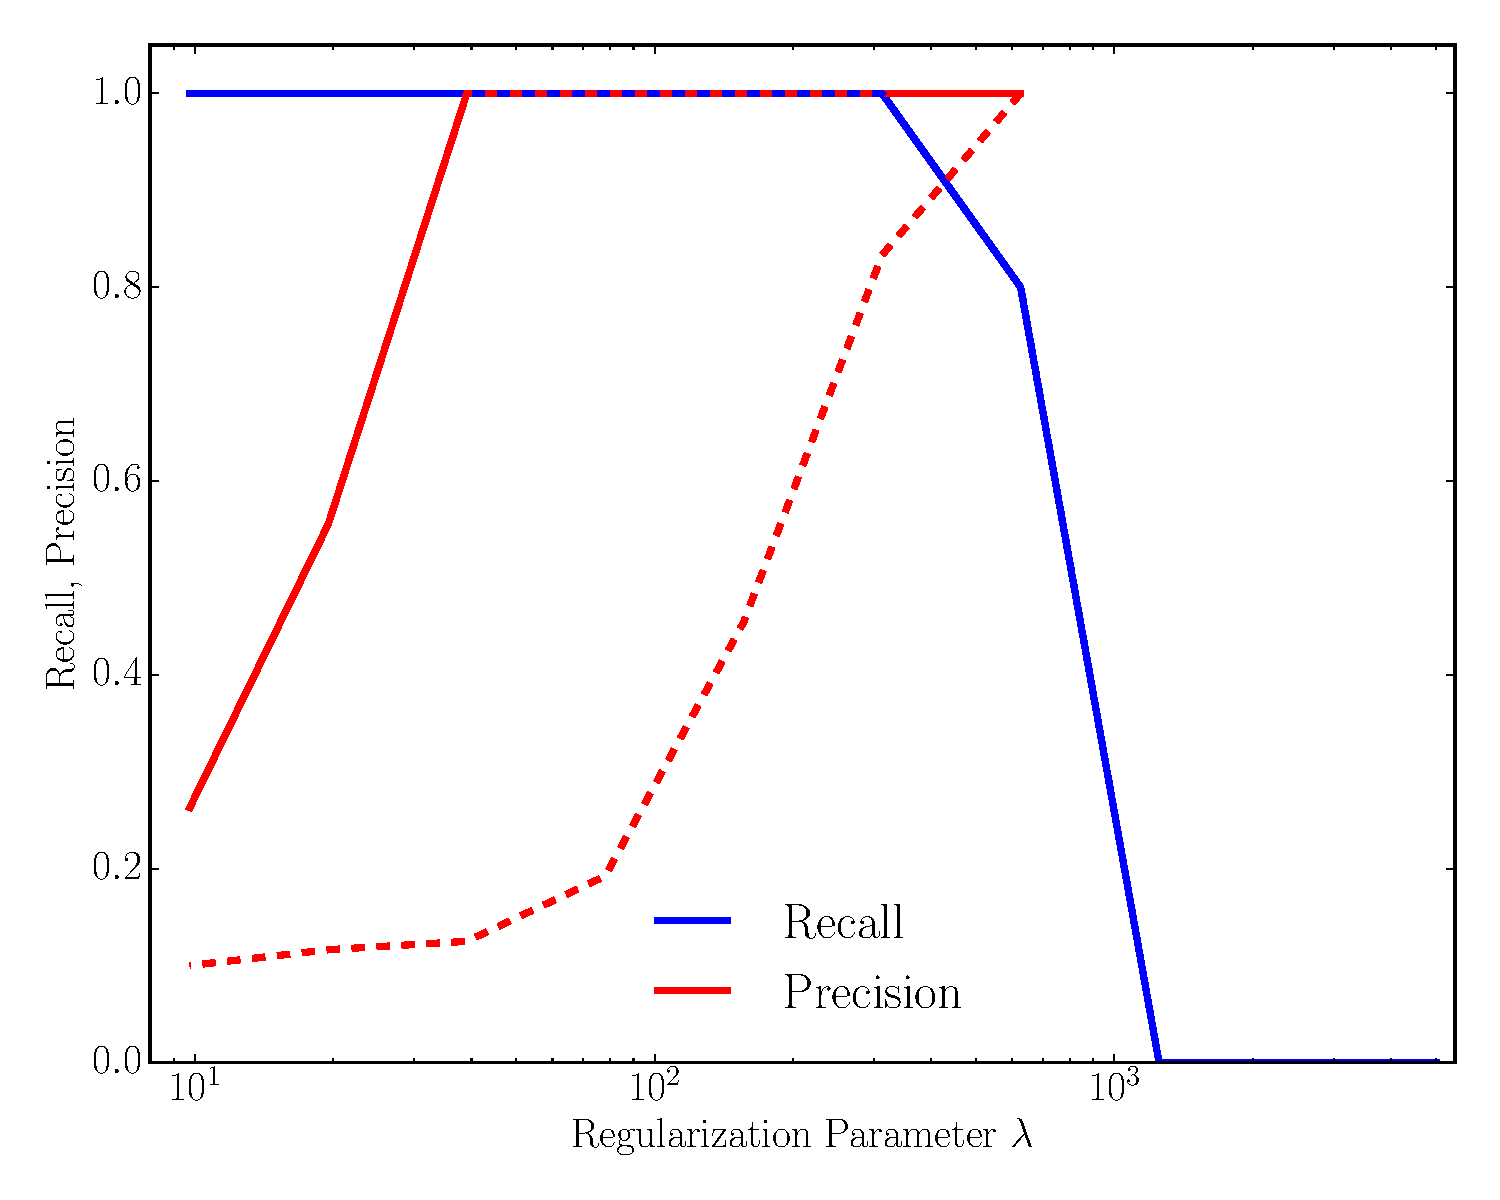
\includegraphics[width=\columnwidth]{synthetic_prec_rec.pdf}
    \caption{Precision (red curves) and recall (blue curves) as a function of the regularization coefficient $\lambda$ over a regularization path.  Solid curves represent data generated with $\sigma = 1$ while dashed curves represent noisy data generated assuming $\sigma = 10$.  For a given $\lambda$, the fitting the noisy $\sigma = 10$ data using the LASSO algorithm yields less precise answers but comparable recall relative to the $\sigma = 1$ data}
    \label{fig:synth_reg}
\end{figure}

For data generated with $\sigma = 1$ (solid curves in Fig.~\ref{fig:synth_reg}), a $\lambda \sim 10^3$ gives perfect precision and recall.  Larger $\lambda$s yield a larger regularization penalty which enforces a sparser solution, causing correct non-zero values to go to 0 resulting in worse recall and precision.  Smaller $\lambda$s have little effect on recall.  The LASSO algorithm tends towards ordinary least squares regression for smaller $\lambda$ and hence is still able to correctly determine the true non-zero values giving the observed perfect recall.  In this regime, however, the reduce penalty term also allows terms in $\hat{\omega}$ that should be 0 to become non-zero due to the regression algorithm overfitting the inherent noise in the data.  The additional non-zero terms arising from overfitting the noise drives the precision down as $\lambda$ decreases as the number of correct non-zeros in $\hat{\omega}$ stays the same while the total number of non-zero terms grows.

\subsubsection*{7.3.2}

I reran the same regularization analysis for the data generated with $\sigma = 10$ (dashed curves in Fig.~\ref{fig:synth_reg}) as I did for the $\sigma = 1$ data over the same $\lambda$ regularization path allowing for a direct comparison of the algorithm's performance for a given $\lambda$.  In general, I found that the recall was relatively unchanged between the two fits for all $\lambda$.  This makes sense since too large a $\lambda$ drives all $\hat{\omega}$ to 0 while smaller $\lambda$ allows for the linear regression to recover the correct non-zero values of $\omega_{true}$.  The precision for the fits on the data generated with $\sigma = 10$, however, was much worse than the fits over the $\sigma = 1$ data for almost all values of $\lambda$.  The enhanced noise in that synthetic dataset makes overfitting an issue and hence underscores the importance of regularization.  At larger $\lambda$, the precision is reasonable as the regularization penalty prevents the LASSO algorithm from overfitting and producing more incorrect non-zero terms in $\hat{\omega}$.  Smaller $\lambda$, however, yield a weaker regularization penalty and hence the algorithm overfits, producing many incorrect non-zero terms in $\hat{\omega}$ in giving poor precision.  

In order to achieve the optimal precision and recall for this noisy data, one should run a regularization path as before while monitoring recall.  Once recall has increased to 1, that $\lambda_{best}$ should be returned as the optimal regularization coefficient.  For $\lambda < \lambda_{best}$, the regularization penalty would be too low allowing noise to produce spurious features yielding incorrect non-zero terms in $\hat{\omega}$.  For the general case where $\omega_{true}$ is not known, one should bias towards larger $\lambda$ for noisy data to prevent overfitting.

\subsection*{7.4: Become a data scientist at Yelp}

Note: The following scripts (attached) include all code used to solve this question: {\tt hw1$\_$7.4.py, regression$\_$utils.py, lasso$\_$utils.py \text{ and } validation.py}.  The script {\tt hw1$\_$7.4.py} produces my answers for this question.  I should note that the regularization path for both the Yelp upvote and star data took of order hours to run to completion so I cache the results as NumPy $.npz$ files that are available upon request.  

To normalize the data for both the upvote and star datasets, for a given dataset, I divided each column (feature) vector by its $l_2$ norm such that each feature vector for the dataset had an $l_2$ norm of unity.  The script I used to normalize the data is {\tt normalize$\_$yelp.py}.

\subsubsection*{7.4.1: Yelp Upvotes}

Following the instructions, I randomly partitioned the data into a training set with $N_{train} = 4000$, a validation set with $N_{val} = 1000$ and a testing set with $N_{test} = 1000$.  For my regularization path, I started at $\lambda_{max} = 2 ||X^{T}(y - \bar{y}) ||_{\infty}$ and decreased $\lambda$ by a factor of 1.25 each iteration for 20 steps.  I found that 20 iterations allowed me to find the minimum of the validation error and also allowed me to see the subsequent validation error increase after its minimum as expected.  After the first step, I initialized each LASSO algorithm with the previous solution.  

Each iteration, I fit the training data with my implementation of the LASSO Coordinate Descent Algorithm 2 to find $\hat{w}$ and $w_0$.  Using the results of the fit, I evaluated the model on the training and validation data and computed the root-mean-squared-error (RMSE) for both.  I also computed the number of nonzeros in the fitted weight vector $\omega$.  The $\lambda$ that yields the minimum validation RMSE after fitting on the training data is the best $\lambda$ and will be used for subsequent model evaluation on the testing data.  The RMSE and number of nonzeros as a function of $\lambda$ along the regularization path are shown in Fig.~\ref{fig:yelp_upvote_rmse} and Fig.~\ref{fig:yelp_upvote_nonzeros}.

\begin{figure}
	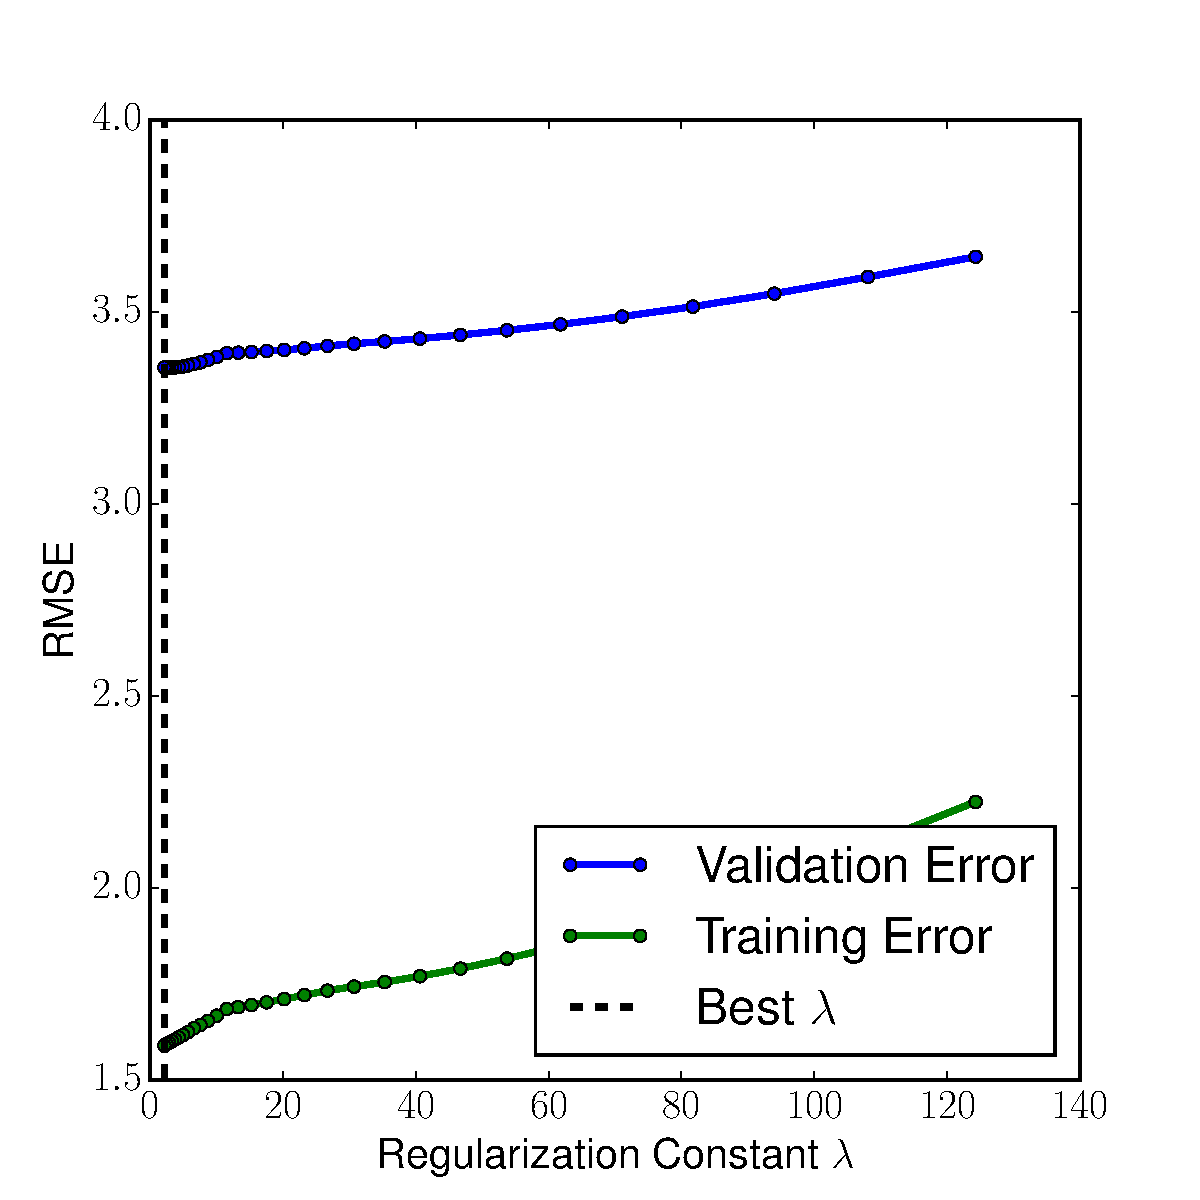
\includegraphics[width=\columnwidth]{upvote_rmse.pdf}
    \caption{Upvote dataset: RMSE for the training set (green) and validation set (blue) as a function of regularization parameter $\lambda$.  The black dashed vertical line corresponds to the minimum validation error and hence optimal $\lambda$.}
    \label{fig:yelp_upvote_rmse}
\end{figure}

\begin{figure}
	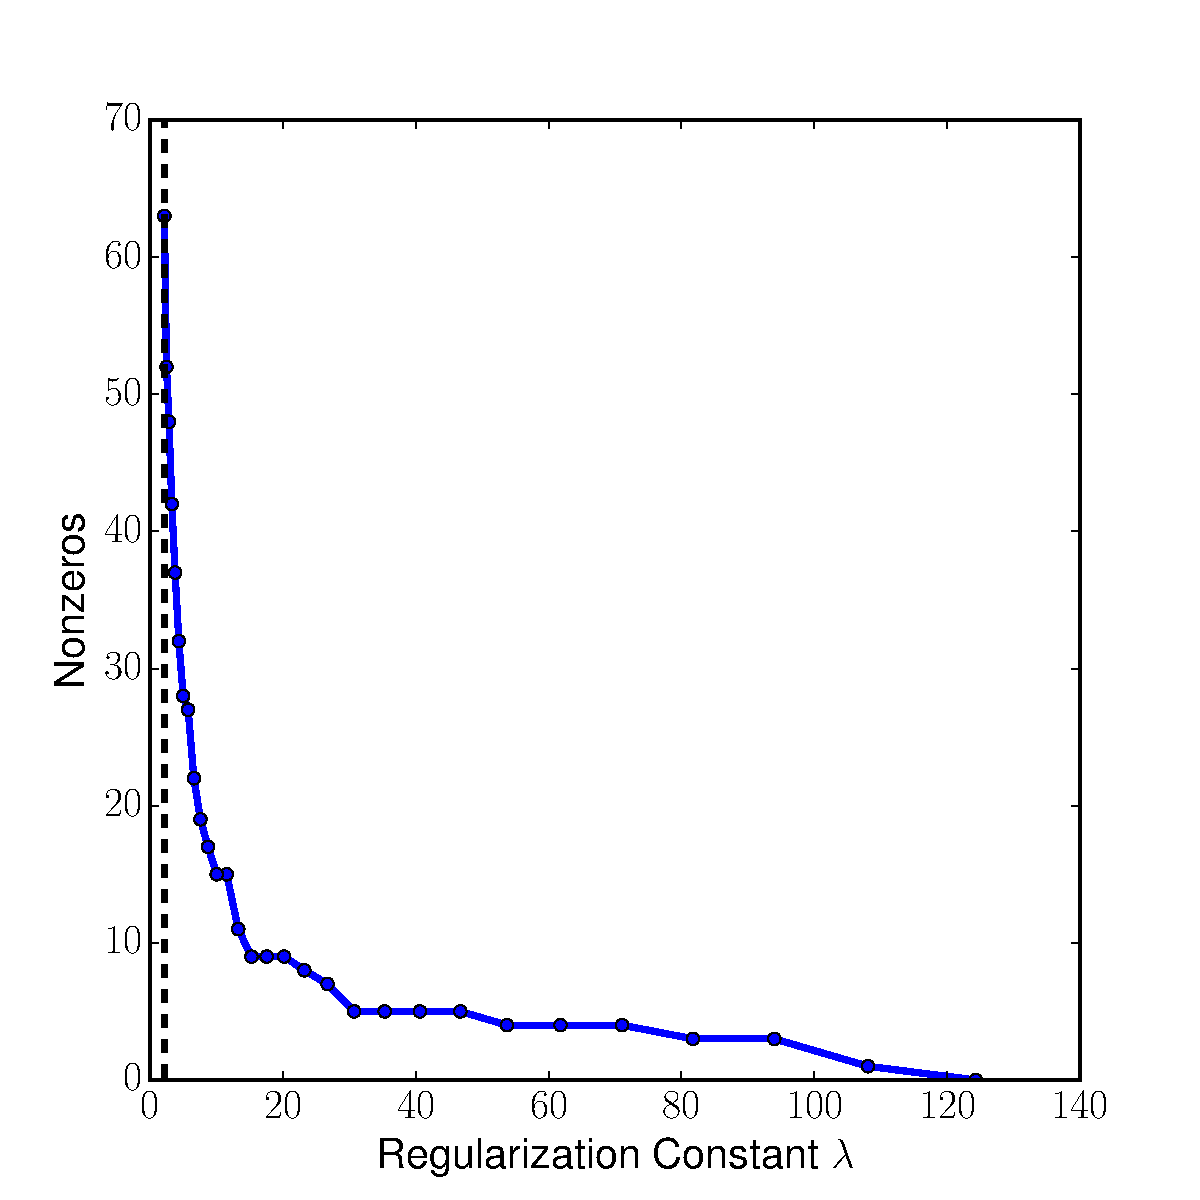
\includegraphics[width=\columnwidth]{upvote_nonzeros.pdf}
    \caption{Upvote dataset: Number of nonzeros in the predicted weight vector $\hat{\omega}$ as a function of regularization parameter $\lambda$.  As before, the black dashed vertical line corresponds to the minimum validation error and hence optimal $\lambda$.}
    \label{fig:yelp_upvote_nonzeros}
\end{figure}

As $\lambda$ decreases, the training error monotonically decreases, likely overfitting the training set at small $\lambda$.  The validation error also decreases with decreasing $\lambda$ but seems to reach a minimum at the best fit $\lambda$ before increasing at the iteration.  As expected, The number of nonzeros increase with decreasing $\lambda$.  The best fit $\lambda$ yields a solution with about 60 nonzero elements.

\subsubsection*{7.4.2}

The best $\lambda$ was selected over the regularization path by fitting on the training set and testing on the validation set.  I found a minimal RMSE of A and B on the training and validation sets, respectively.  The best $\lambda$ was that which yielded the smallest validation set error.  From this procedure, I determined $\lambda_{best} = X$ for the Yelp upvote data.  Using this $\lambda_{best}$, I refit the training data and using the resultant weight vector, I evaluated the model on the testing data and got an RMSE of Z.  As expected, my training set error was less than my validation set error which was less than my testing set error.  This makes sense as any model will likely tend to preform worse on new data as during the training process, model parameters, e.g. $\omega$, $w_0$, are optimizing over the training data.

\subsubsection*{7.4.3}

In the table below, I shown the 10 features with weights largest in magnitude.

\begin{table}
	\centering
	\caption{Top 10 Upvote Weights by Magnitude}
	\begin{tabular}{ccc} 
		\hline
		Rank & Weight Name & Weight Coefficient \\
		\hline
		1 & 0 & 0.00383 \\
		2 & 0.001 & 0.00383 \\
		3 & 0.05 & 0.00383 \\
		4 & 0.1032 & 0.00383 \\
		5 & 0.25 & 0.00383  \\ 
		6 & 0.1032 & 0.00766  \\
		7 & 0.1032 & 0.00192  \\
		8 & 0.1032 & 0.00574  \\
		9 & 0.1032 & 0.00383 \\
		10 & 0.1032 & 0.00383 \\
		\hline
	\end{tabular}
	\label{tab:top_upvotes}
\end{table}

Discussion.  What is an upvote?

\subsubsection*{7.4.4}

Repeat above.  What is a star?

\begin{figure}
	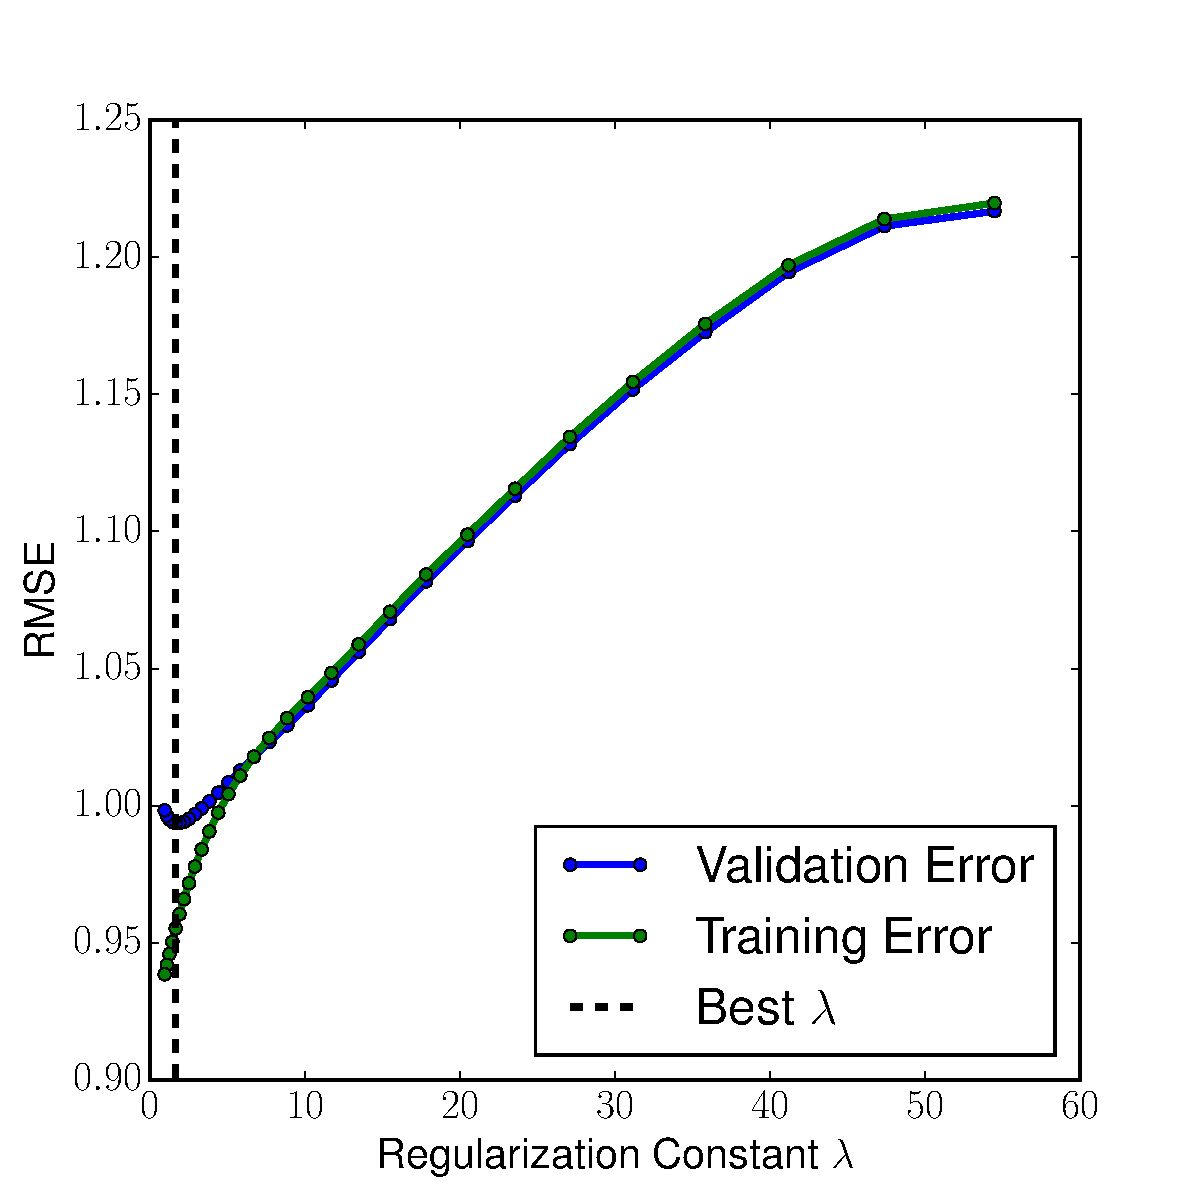
\includegraphics[width=\columnwidth]{star_rmse.pdf}
    \caption{Star dataset: RMSE for the training set (green) and validation set (blue) as a function of regularization parameter $\lambda$.  The black dashed vertical line corresponds to the minimum validation error and hence optimal $\lambda$.}
    \label{fig:yelp_star_rmse}
\end{figure}

\begin{figure}
	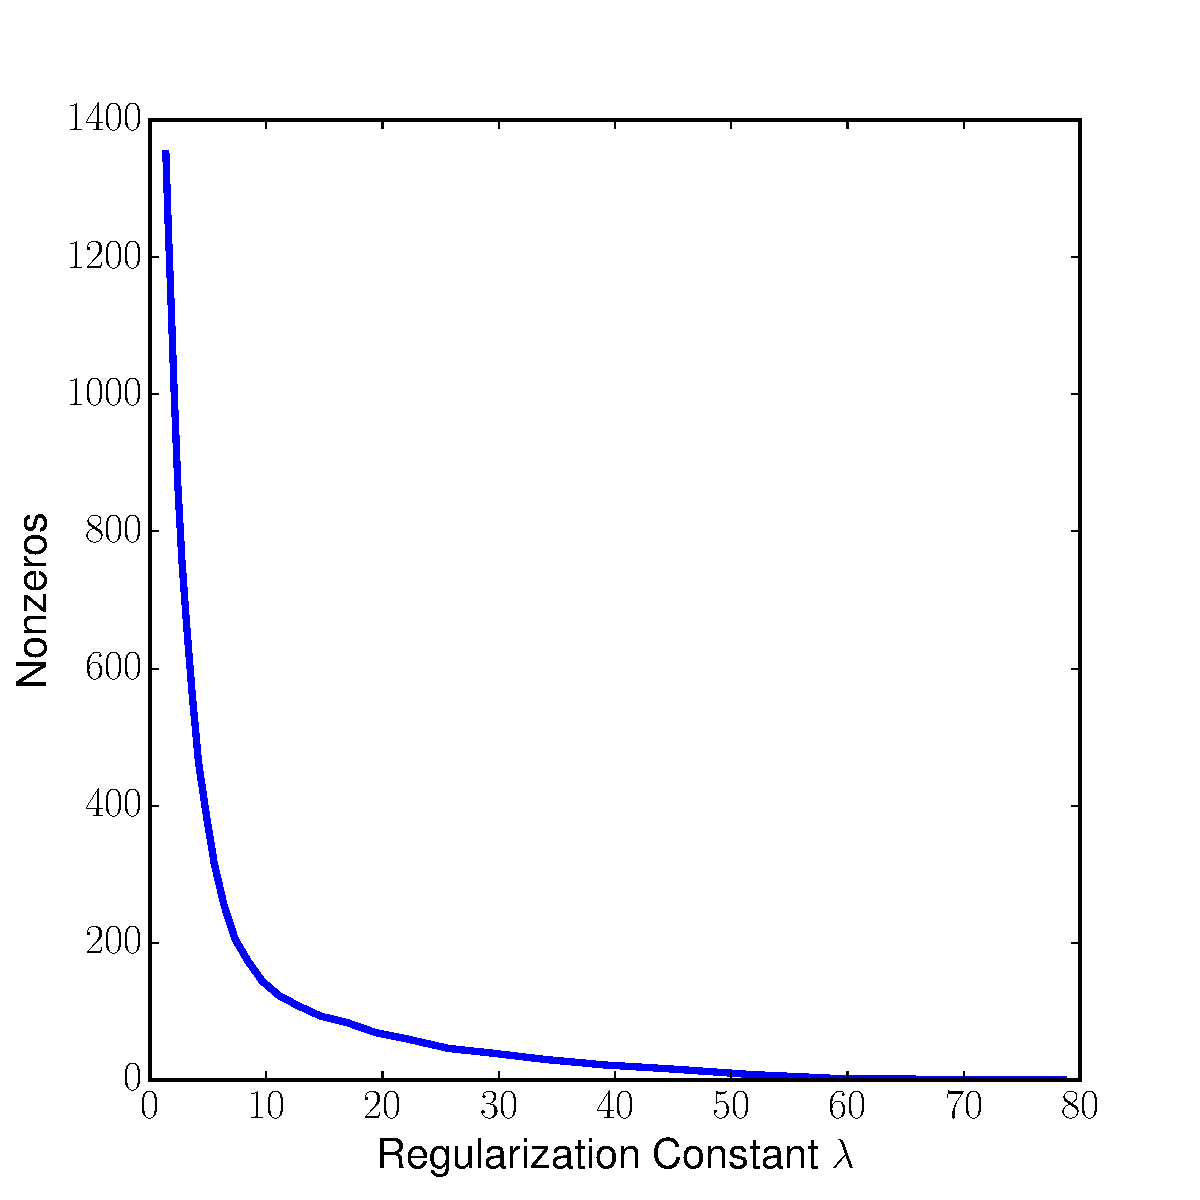
\includegraphics[width=\columnwidth]{star_nonzeros.pdf}
    \caption{Star dataset: Number of nonzeros in the predicted weight vector $\hat{\omega}$ as a function of regularization parameter $\lambda$.  As before, the black dashed vertical line corresponds to the minimum validation error and hence optimal $\lambda$.}
    \label{fig:yelp_star_nonzeros}
\end{figure}

DISCUSS trends in plots.

\begin{table}
	\centering
	\caption{Top 10 Stars Weights by Magnitude}
	\begin{tabular}{ccc} 
		\hline
		Rank & Weight Name & Weight Coefficient \\
		\hline
		1 & 0 & 0.00383 \\
		2 & 0.001 & 0.00383 \\
		3 & 0.05 & 0.00383 \\
		4 & 0.1032 & 0.00383 \\
		5 & 0.25 & 0.00383  \\ 
		6 & 0.1032 & 0.00766  \\
		7 & 0.1032 & 0.00192  \\
		8 & 0.1032 & 0.00574  \\
		9 & 0.1032 & 0.00383 \\
		10 & 0.1032 & 0.00383 \\
		\hline
	\end{tabular}
	\label{tab:top_stars}
\end{table}


Note: On this question, I collaborated with Matt Wilde, Serena Liu, and Janet Matsen.

\end{document}